\documentclass[a4paper,11pt, twocolumn]{article}
\usepackage[margin=0.8in]{geometry}
\usepackage{xcolor}
\usepackage{graphicx} %package to manage images
\graphicspath{ {./images/} }
\usepackage{amsmath}
\usepackage{amssymb}

\title{A2-5 Signal Conversion}
\author{Revision sheet}
\date{}

\usepackage{fancyhdr}
\pagestyle{fancy}
\fancyhead{} % clear all header fields
\renewcommand{\headrulewidth}{0pt} % no line in header area
\fancyfoot{} % clear all footer fields
\renewcommand{\footrulewidth}{0.4pt}
\fancyfoot[C]{\thepage} % page number in centre of the page
\fancyfoot[R]{\footnotesize Thomas Boxall \\ Images from WJEC E-Book} % right hand footer has author name on top line and images reference on bottom line
\fancyfoot[L]{\footnotesize A2-5 Signal Conversion \\ Revision sheet} % left hand footer has title of document on top line and 'Revision Sheet' on bottom line


\begin{document}

\maketitle
\thispagestyle{fancy}

% CONTENTS OF THE REVISION SHEET HERE
\section{Analogue To Digital Converters}
Audio starts out as an analogue signal, gets processed by a digital signal processor then gets turned back to analogue so we can hear it. 
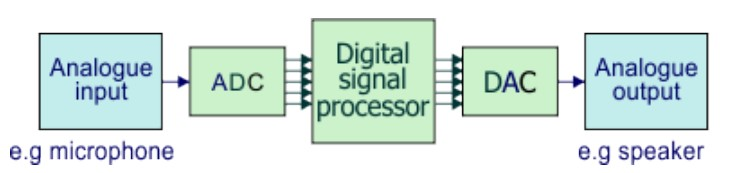
\includegraphics[width=\linewidth]{audioSystemBD.jpg}
\subsection{Flash ADC}
Flash Analogue To Digital Converters are very quick. They use comparators and the following two comparator rules as the fundamentals to their operation
\begin{align*}
    V_{IN} > V_{REF} & \therefore V_{OUT} = +V_{SAT}\\
    V_{IN} < V_{REF} & \therefore V_{OUT} = -V_{SAT}
\end{align*}
where $V_{IN}$ is the non-inverting input and $V_{REF}$ is the inverting input.
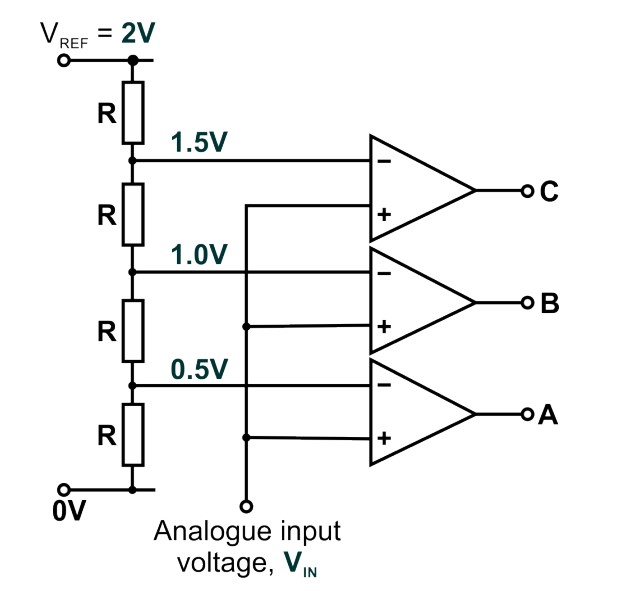
\includegraphics[width=\linewidth]{smolFlash.jpg}
The circuit diagram above is for a basic flash ADC (missing a component). The comparators will turn on if $V_{IN}$ is above the reference voltage provided to their inverting input by the resistor ladder. The inputs and outputs have the following relationship
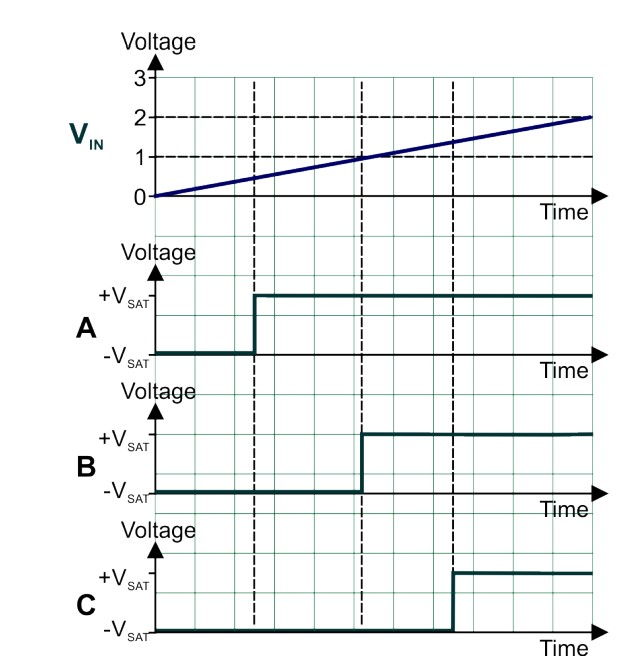
\includegraphics[width=0.9\linewidth]{smolFlashGraph.jpg}
\subsubsection{3-Bit Flash ADC}
In the example below, a `Priority Encoder' has also been added to the circuit diagram. This will generate a binary sequence based off of the highest input value it receives.
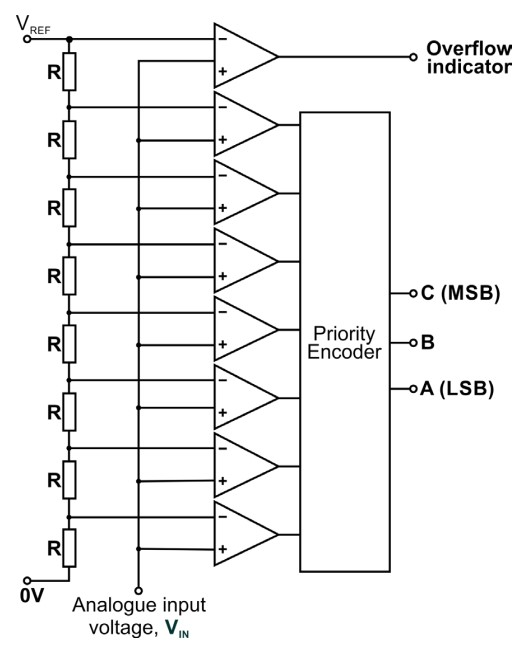
\includegraphics[width=\linewidth]{3bitFlash.jpg}
The diagram above also has an additional comparator - used to indicate if $V_{IN}$ is out of range.
\subsection{Digital Ramp ADC}
This is a much slower ADC (than the Flash ADC), due to this, it isn't used in audio but is used in voltmeters. Block diagram for Digital Ramp ADC shown below.
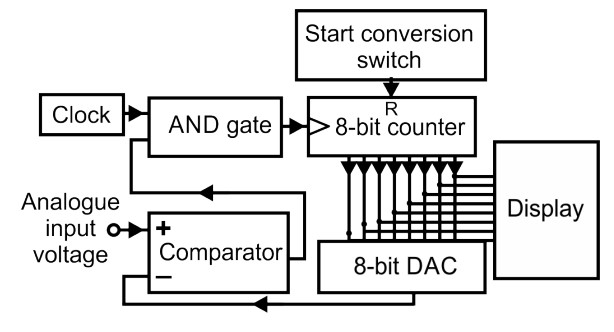
\includegraphics[width=\linewidth]{rampADC.jpg}
When the start conversion switch is pressed, the counter is reset to 0. The counter then begins to count up, feeding a higher number to the DAC - this increases the DACs $V_{OUT}$ in a stepped waveform. The clock signal will only go through if the output of the comparator is 1. This counting continues until DAC $V_{OUT} > V_{IN}$ then the AND gate stops allowing pulses through so the counting stops and the value can be read off. The ADC does this cycle very quickly. If it overflows, it will continue looping around counting - without indicating this to the user.
\subsubsection{Comparison With Flash ADC}
Flash ADC is faster. Flash ADC is much more complex. Flash ADC is more expensive.
\subsection{Equations}
There are a number of equations needed for ADCs, mostly only applicable to the Flash ADC.
\subsubsection{Resolution}
\textit{The resolution is the minimum change in input voltage that will guarantee a change in the output voltage} (basically, how sensitive the ADC is).
$\displaystyle resolution = \frac{input\ voltage\ range}{2^{number\ of\ bits}}= \frac{V_{REF}}{2^n}$\\
\subsubsection{Average Quantization Error}
$\displaystyle Average\ quantization\ error = \frac{resolution}{2}$

\section{Digital To Analogue Converters}
DACs are based off of an op-amp summing amplifier. A recap is shown below.
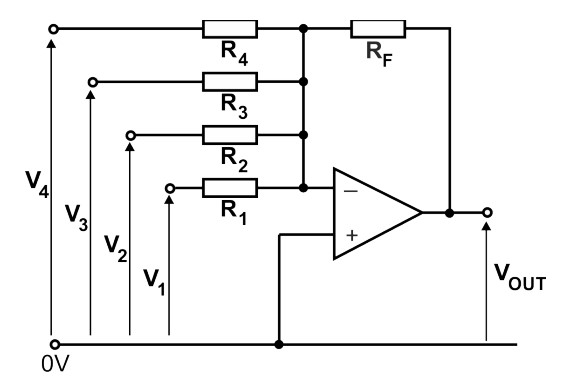
\includegraphics[width=\linewidth]{op-ampSumming.jpg}
$\displaystyle V_{OUT} = -R_{f} \left(\displaystyle \frac{V_1}{R_1} + \frac{V_2}{R_2} + \frac{V_3}{R_3} + \frac{V_4}{R_4} \right)$\\
$\displaystyle Input_n\ gain = \frac{-R_f}{R_{n}}$
\subsection{Converting To DAC}
The output of the summing amplifer is inverted compared to the input. This is a problem! To solve this,we add another inverting amplifer with gain $-1$, which will invert the signal to the right way around.
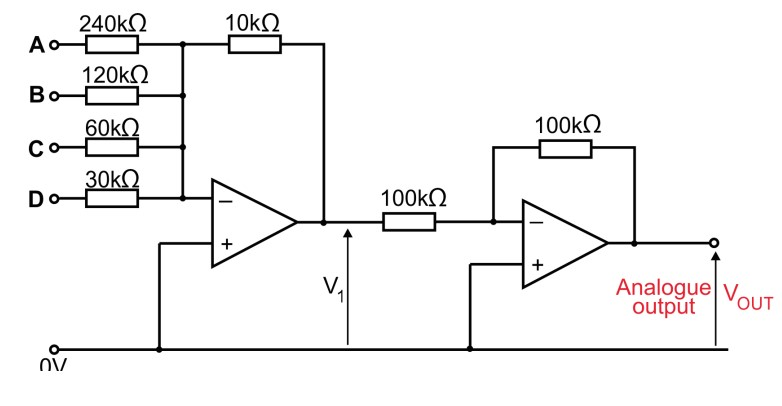
\includegraphics[width=\linewidth]{fullDAC.jpg}
In the circuit diagram above, D is the most significant bit and A is the least significant bit.
The gain of the individual inputs can be calculated as follows
\begin{align*}
    G_D &= \frac{-10}{30} = \frac{-1}{3}\\
    G_C &= \frac{-10}{60} = \frac{-1}{6}\\
    G_B &= \frac{-10}{120} = \frac{-1}{12}\\
    G_A &= \frac{-10}{240} = \frac{-1}{24}
\end{align*}
The relationship between the inputs and output can be shown in a table as follows
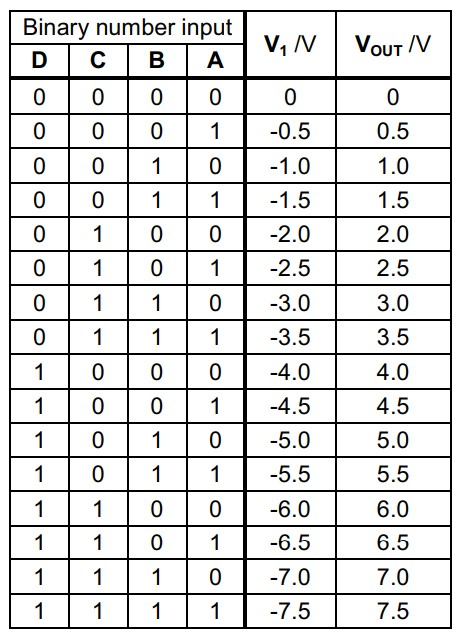
\includegraphics[width=\linewidth]{dacBinary.jpg}
as well as on a graph, which also shows the step size.
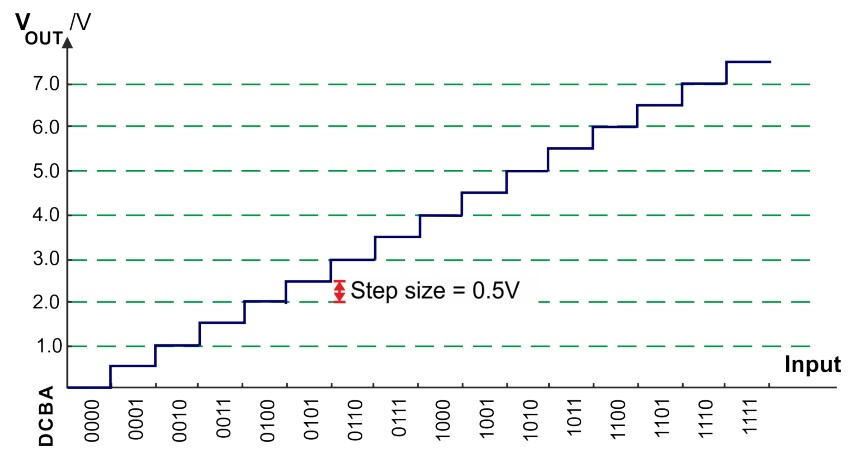
\includegraphics[width=\linewidth]{dacGraph.jpg}
The step-size can also be calculated using the following equation (this is \textbf{NOT} in the formula book)\\
$\displaystyle stepSize = V_{L1} \frac{R_F}{R_{LSB}}$\\
where $V_{L1}$ is the logic 1 voltage and $R_{LSB}$ is the resistor value of the least significant bit. The number of steps $= 2^n -1$ where $n$ is the number of bits.

\section{Digital Audio Systems}
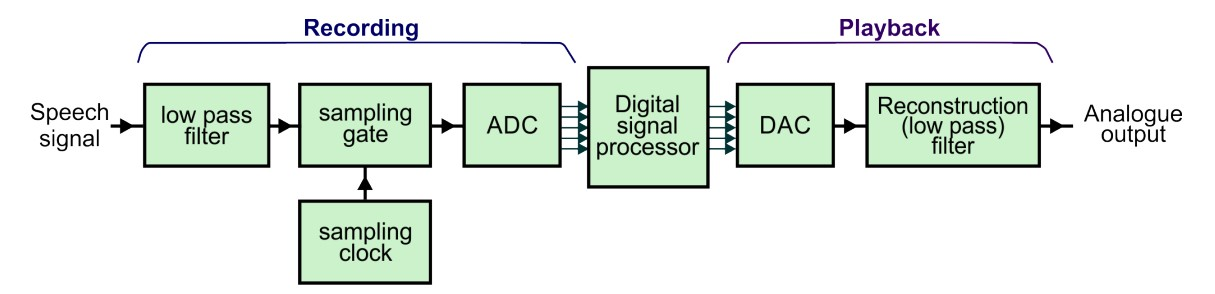
\includegraphics[width=\linewidth]{digitalAudioSystemBD.jpg}
\subsection{Sampling Gate}
Digital audio is `sampled' at set frequencies. The quality of the final recording will depend on how frequent this sampling is. 
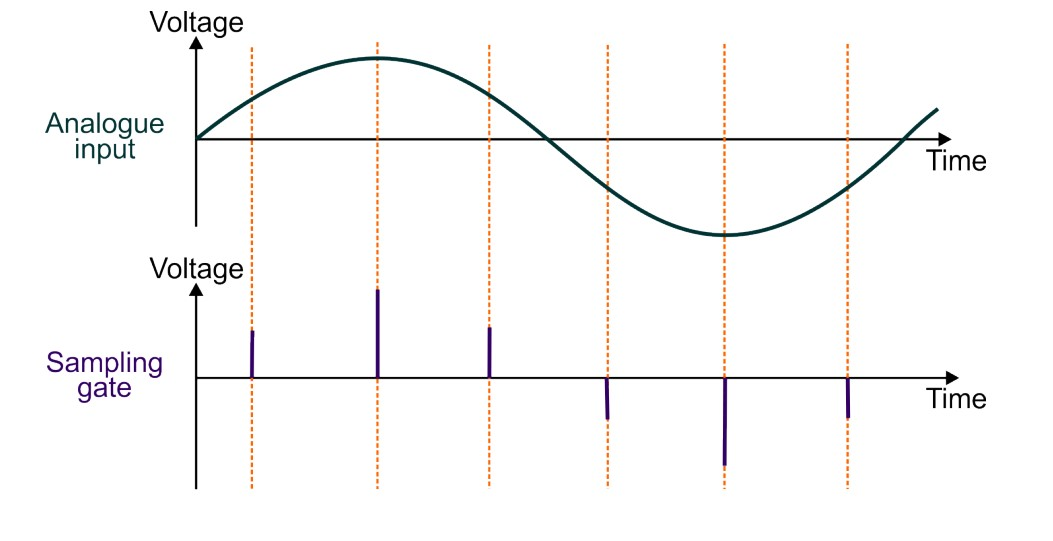
\includegraphics[width=\linewidth]{dasSamplingGate.jpg}
The sampling frequency can be calculated using the following equation\\
$f = \frac{1}{T} \displaystyle$\\
After being processed by the sampling gate, the signal is quantized in the time domain and the voltage is still analogue. 
\subsubsection{Aliasing}
When a sample rate is too low, the signal changes. This is called aliasing. To avoid aliasing, we can use the Nyquist Theorem. The Nyquist theorem states that the sample frequency must be at least 2 times the maximum signal frequency.
\subsection{Low Pass Filter}
The low pass filter prevents aliasing as it blocks frequencies $> \frac{1}{2}f_s$
\subsection{Bit-Rate}
Bit Rate is the number of bits per second. It can be calculated using the following equation.\\
$bit\ rate = f_s \times num\ bits\ per\ sample$ where $f_s$ is the sample frequency. 
\subsection{File Size}
The file size is the size of the final file. It can be calculated using the following equation.\\
$file\ size = bit\ rate \times sampling\ time$
\subsection{Outputs}
The DAC outputs a staircase waveform, this is passed through another LPF which smoothens out the waveform. The Low Pass Filter filters out the high frequencies which in square waves (due to Fourier Analysis).
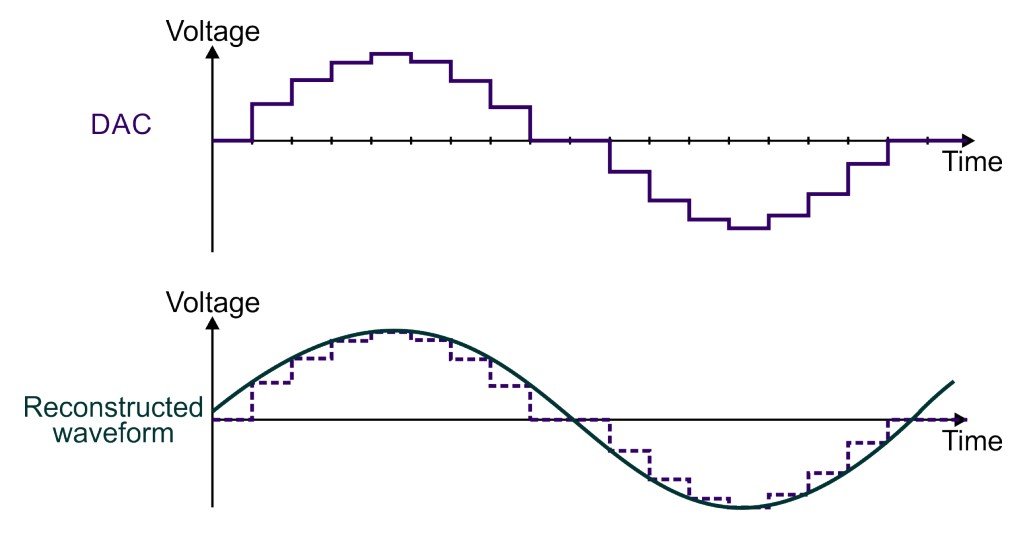
\includegraphics[width=\linewidth]{output.jpg}


\end{document}